\documentclass[tikz]{standalone}

\usepackage{tikz}
\usepackage{pgfplots}
\pgfplotsset{compat=1.16}

\usetikzlibrary{math}
\usetikzlibrary{arrows.meta}


\begin{document}
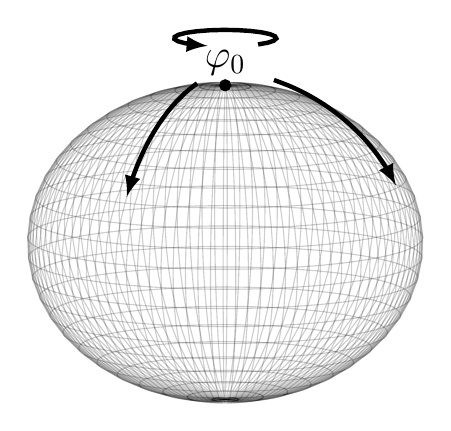
\begin{tikzpicture}
    \begin{axis}[
        axis lines=center, 
        ticks=none, 
        view/h=120, 
        view/v=10, 
        axis line style={draw=none},
        every node near coord/.append style={font=\Large}
    ]
    % Sphere
    \addplot3[%
    opacity = 0.1,
    mesh,
    black,
    z buffer = sort,
    samples = 50,
    variable = \u,
    variable y = \v,
    domain = 0:180,
    y domain = 0:360,
    ]
    ({cos(u)*sin(v)}, {sin(u)*sin(v)}, {cos(v)});
    \addplot3 [mark=*, nodes near coords=$\varphi_0$] coordinates {(0, 0, 1)};
    \addplot3[%
    -latex,
    domain=15:65,
    samples=10,
    samples y=0,
    no marks,
    smooth,
    ultra thick,
    ]
    ({0}, {1.1*sin(x)}, {1.1*cos(x)});
    \addplot3[%
    -latex,
    domain=15:65,
    samples=10,
    samples y=0,
    no marks,
    smooth,
    ultra thick,
    ]
    ({1.1*sin(x)}, {0}, {1.1*cos(x)});
    ]
    ({sin(x)}, {-sin(x)}, {cos(x)});
    \addplot3[%
    latex-,
    ultra thick,
    samples = 20,
    samples y=0,
    variable = \u,
    variable y = \v,
    domain = -280:20,
    ]
    ({sin(15)*sin(u)}, {sin(15) * cos(u)}, {1.3});
    \end{axis}
\end{tikzpicture}
\end{document}
